% --------------------------------------------
\documentclass{Arquivos/TrabalhoAcademico} 
% --------------------------------------------
% Dados Pré-Textuais
% --------------------------------------------
\titulo{Projeto de Pesquisa:\\ {\large Modelo Conforme Normas UFT/ABNT}}

\autor{\WenesTex Aquino}

\orientador{\WenesTex Gomes Aquino}
\coorientador{Beltrano Vitória Almeida}

\local{Arraias -- TO}
\data{2025, v-2.0}

\instituicao{%
  Universidade Federal do Tocantins \\
  Campus Universitário de Palmas \\
  Curso de Licenciatura em Computação
}


\tipotrabalho{Projeto de Pesquisa}


\preambulo{Projeto de Pesquisa apresentado como 
    parte dos requisitos para avaliação na Universidade 
    Federal do Tocantins. Este modelo foi adaptado 
    e personalizado com ajustes visuais e estruturais, 
    servindo também para testar o espaço disponível 
    utilizada nessa contracapa. Por \WenesTex.}



\begin{document}
\nocite{*}


\pretextual % =================================


\folhaderosto
\contracapa


\listaDeFiguras
\listaDeTabelas


\begin{siglas}
    \item[CPU] Unidade Central de Processamento
    \item[RAM] Memória de Acesso Aleatório
    \item[SSD] Unidade de Estado Sólido (Solid State Drive)
\end{siglas}


\begin{simbolos}
    \item[$\alpha$] Alfa (Ângulo, Coeficiente de Temperatura)
    \item[$\beta$] Beta (Ângulo, Ganho de Corrente do Transistor)
    \item[$\sum$] Somatório (Usado em Séries Matemáticas e Estatística)
\end{simbolos}

\Sumario


\textual % ==================================


\capituloCentralizado{Introdução}


\chapter{Desenvolvimento}
\section{Desenvolvimento}


\chapter{Considerações finais}
\section{Conclusão}


\postextual % ==================================


\capituloCentralizado{Referências}
\printbibliography[heading=none]


\paginaDivisoria{APÊNDICES}
\inicioApendices
\chapter{Apêndice}


\paginaDivisoria{ANEXOS}
\inicioAnexos
\chapter{Anexo}

\begin{table}[ht]
    \centering
    \caption{Tabela estilosa 5×5}
    \label{tab:estilosa}
    \begin{tabular}{ccccc}
        \toprule
        Col 1 & Col 2 & Col 3 & Col 4 & Col 5 \\
        \midrule
        A1 & B1 & C1 & D1 & E1 \\
        A2 & B2 & C2 & D2 & E2 \\
        A3 & B3 & C3 & D3 & E3 \\
        A4 & B4 & C4 & D4 & E4 \\
        A5 & B5 & C5 & D5 & E5 \\
        \bottomrule
    \end{tabular}
\end{table}

\begin{figure}[ht]
    \centering
    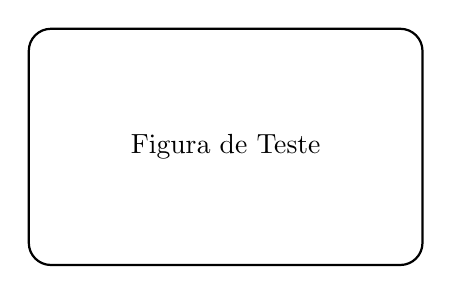
\begin{tikzpicture}
        \draw[rounded corners=8pt, thick] (0,0) rectangle (5,3);
        \node at (2.5,1.5) {Figura de Teste};
    \end{tikzpicture}
    \caption{Figura de teste estilizada}
    \label{fig:teste-estilosa}
\end{figure}


\end{document} 